The previous chapter on finite state machines provided an introduction into high-level robot behavior specification. Another important topic along this thread is \textit{sequential decision making}\cite{Bertsekas2019}, where the robot must make a series of decisions to accomplish an objective in an optimal way. This chapter provides an introduction to fundamental topics in decision making, including for problems where there is some uncertainty (e.g. uncertainty about the robot's state or about the environment).

\notessection{Sequential Decision Making}
In addition to the motion planning and control problems discussed in earlier chapters (which focus on low-level tasks), there exist a broad range of situations where higher-level autonomous decision making is required. For example when deciding whether it is time for a self-driving car to cross an intersection, or whether a robot should first complete task A or task B.
Two of the fundamental challenges associated with robotic decision making are that \textit{sequences} of decisions must be made (which requires reasoning about future actions and observations) and that uncertainty may exist in the operating environment. This chapter presents a modeling framework for addressing decision making problems and will also introduce \textit{dynamic programming}, a fundamental approach for solving these problems .


\subsection{Deterministic Decision Making Problem}
The standard mathematical formulation for decision making problems includes several components: a model of the robot's behavior, a set of admissible controls, and a cost function. This set of components is quite similar to the components used in trajectory optimization problems discussed in previous chapters, however decision making problems are generally represented in \textit{discrete-time} rather than in \textit{continuous-time}\footnote{There is a continuous-time formulation, known as the Hamilton–Jacobi–Bellman formulation.}.

In the deterministic decision making problem, the model of the robot is expressed in \textit{discrete-time} as:
\begin{equation} \label{eq:detmodel}
\x_{k+1}= f_k(\x_k, \bu_k), \quad k = 0, \dots, N-1,
\end{equation}
where $\x$ is the robot's state, $\bu$ is the control, $f_k$ defines how the robot's state changes at time step $k$, and $N$ is an integer that defines a finite planning horizon for the decision making problem. There are generally no restrictions on how the functions $f_k$ are defined, they could come from a physics-based dynamics/kinematics model or even a higher-level state transition model similar to the finite state machine from the previous chapter.

It is also generally assumed that only some control actions are admissible at a given state, which denoted by the set $\mathcal{U}(\x_k)$. For example a car may only have an option to turn left or right when it is at an intersection.
Therefore the control constraints for the robot at time step $k$ are given by:
\begin{equation} \label{eq:SDMPconstraints}
\bu_k \in \mathcal{U}(\x_k).
\end{equation}
Again, there are generally no restrictions on how the set of admissible control is defined. For example $\mathcal{U}(\x_k)$ could be a finite set of actions, it could be a convex region of allowable inputs, etc.

The cost function is assumed to be \textit{additive}, and is defined as:
\begin{equation} \label{eq:detcost}
J(\x_0, \bu_0, \dots, \bu_{N-1}) = g_N(\x_N) + \sum_{k=0}^{N-1} g_k(\x_k, \bu_k),
\end{equation}
where $g_N$ is a terminal state cost function and $g_k$ for $k=0,\dots,N-1$ are stage cost functions. These individual cost functions are also not restricted to a particular form (e.g. convex, differentiable, etc.).

\begin{definition}[Deterministic Decision Making Problem]
The deterministic decision making problem can be expressed for the system model \eqref{eq:detmodel}, control constraints \eqref{eq:SDMPconstraints}, and cost function \eqref{eq:detcost} as:
\begin{equation} \label{eq:dproblem}
J^*(\x_0) = \underset{\bu_k \in \mathcal{U}(\x_k), k=0,\dots,N-1}{\min} J(\x_0, \bu_0, \dots, \bu_{N-1}).
\end{equation}
\end{definition}

Notice that this problem is used to compute an \textit{open-loop} control sequence $\{\bu_0, \dots, \bu_{N-1}\}$ given an initial condition $\x_0$, which is similar to the trajectory optimization problems seen in earlier chapters. However, this problem is generally quite hard to solve since there is no guarantee that the model \eqref{eq:detmodel} and cost function \eqref{eq:detcost} have any particular structure that can be leveraged to make the optimization problem amenable to numerical optimization algorithms. While it is theoretically possible to solve the problem through a brute force search over all possible combinations of sequences $\{\bu_0, \dots, \bu_{N-1}\}$, this leads to a combinatorial explosion of options and is therefore not possible in practical settings (except of course for very small problems).

\subsubsection{Principle of Optimality (Deterministic)}
Fortunately, there is in fact an underlying structure to the deterministic decision making problem that can be leveraged to make the problem easier to solve. This structure is commonly referred to as the \textit{principle of optimality}.
\begin{figure}[ht]
    \centering
    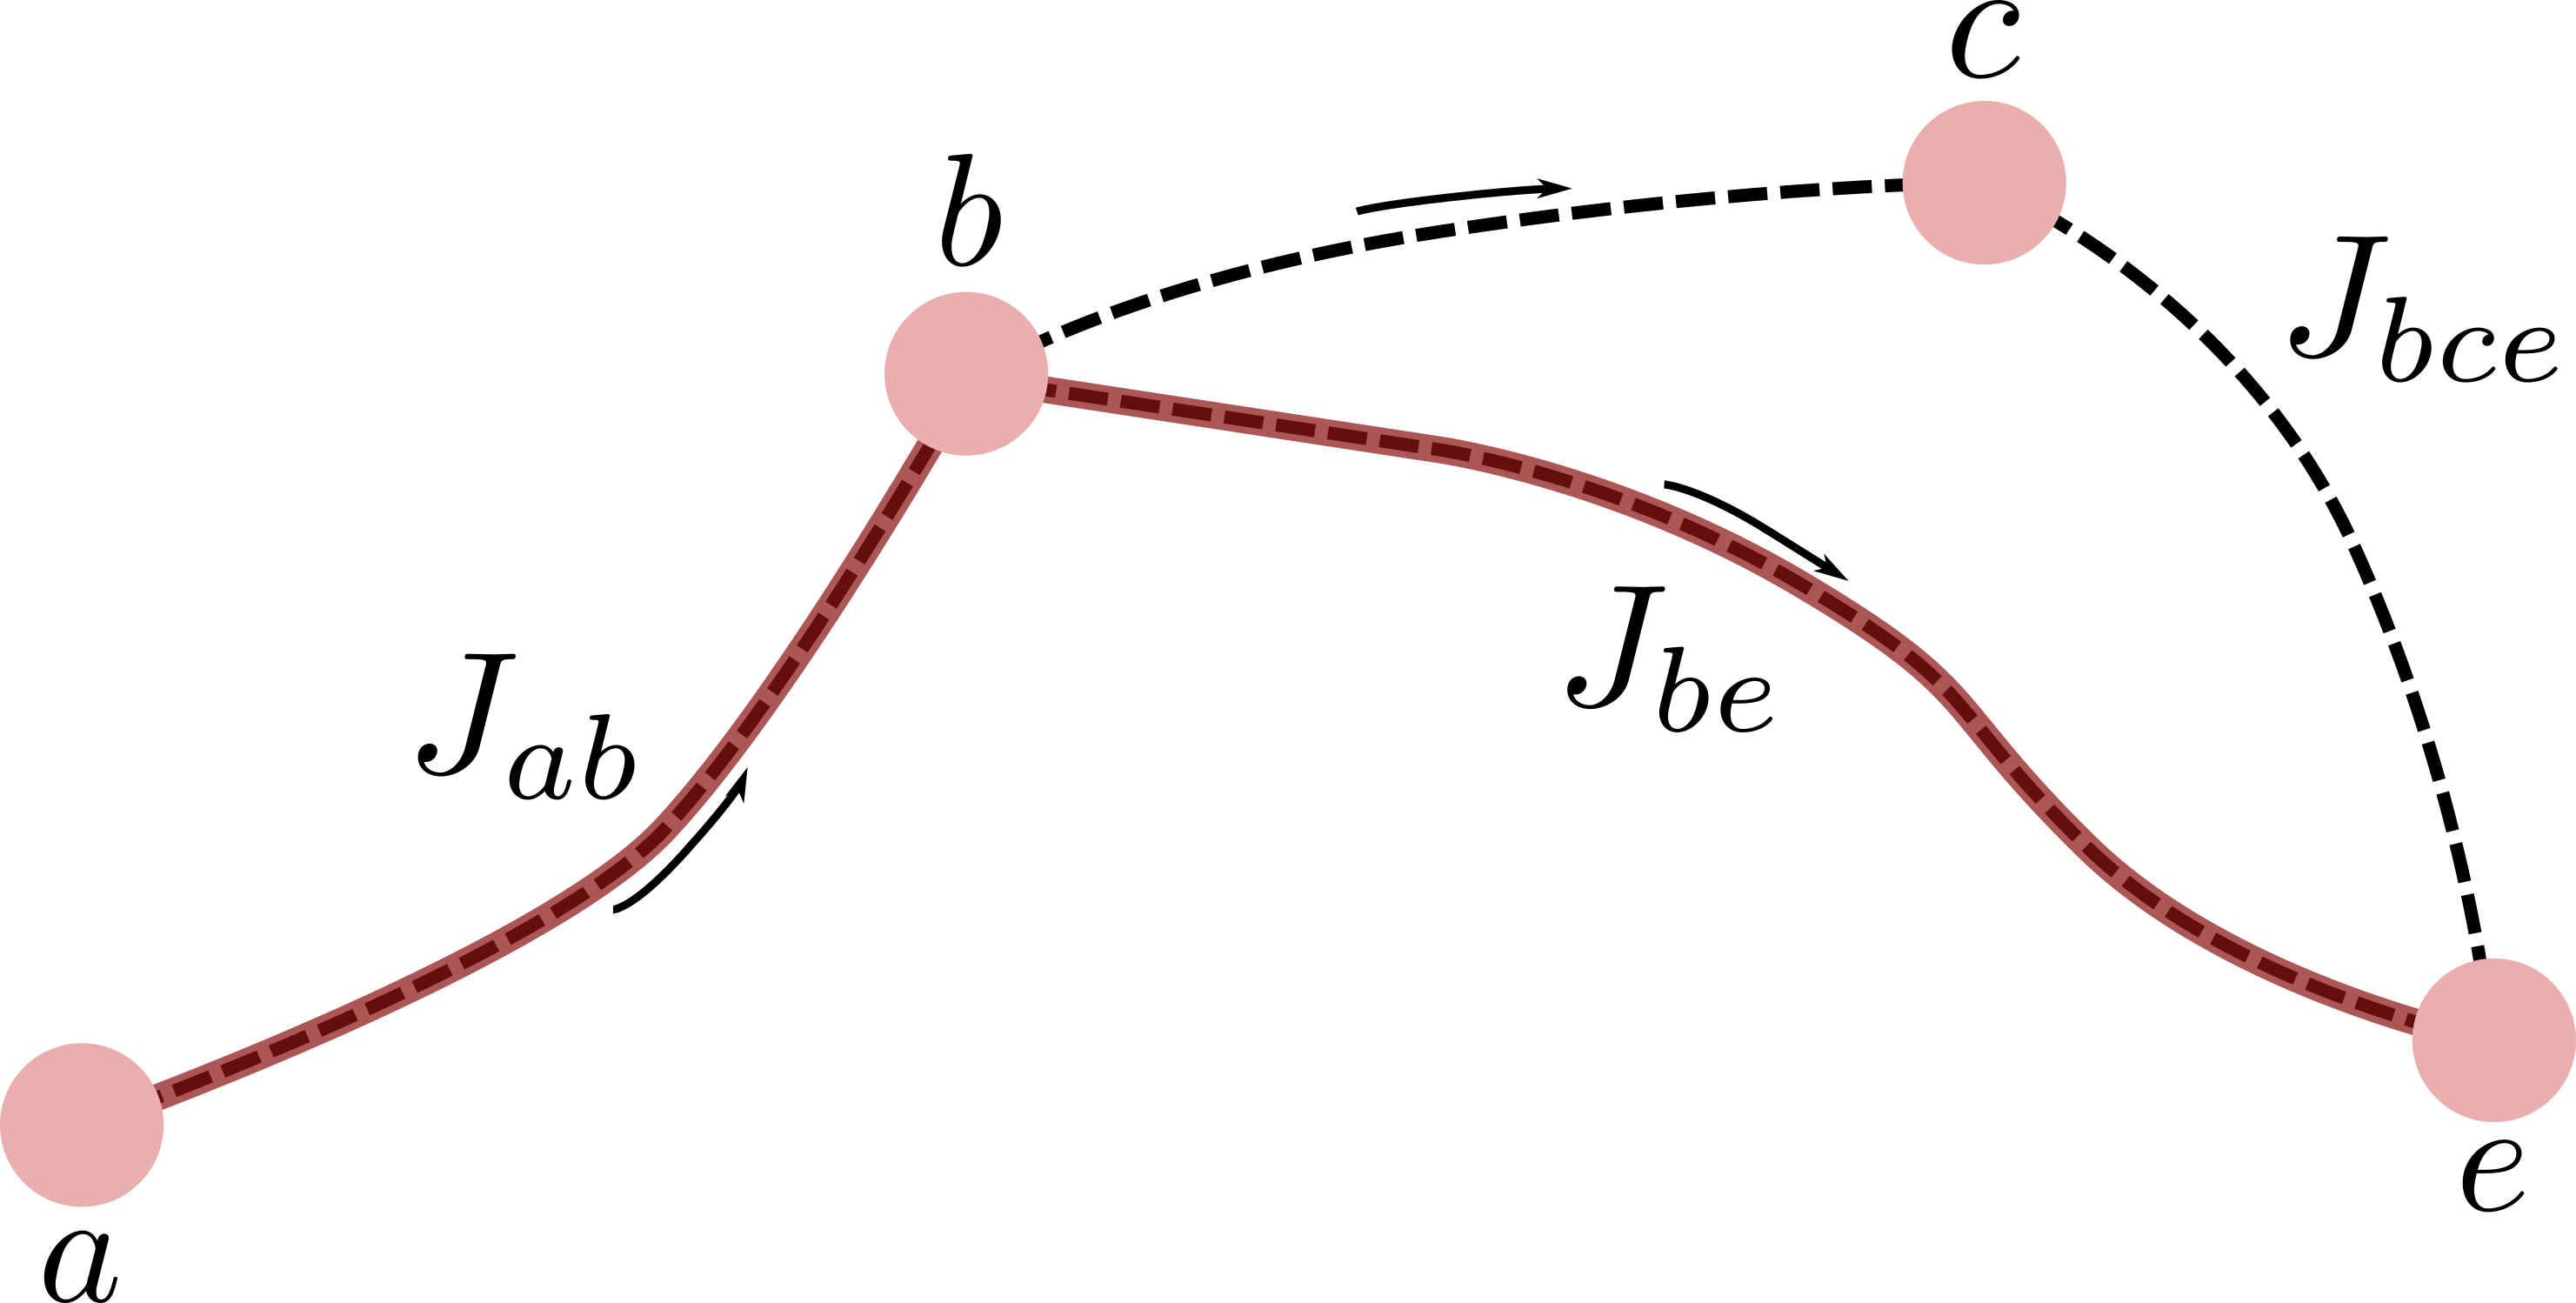
\includegraphics[width=0.5\textwidth]{tex/figs/ch22_figs/princopt1.png}
    \caption{Starting from point $a$, let the green path $a-b-e$ be the optimal path from $a$ to $e$, with a total cost of $J^*_{ae} = J_{ab}+J_{be}$. The principle of optimality in this case says that the path $b-e$ must therefore be the optimal path when starting from point $b$. This can be proven by contradiction, since if the path $b-c-e$ had a lower cost than path $b-e$ (i.e. $J_{bce} < J_{be}$), then the original path $a-b-e$ cannot be optimal!}
    \label{fig:princopt1}
\end{figure}

The principle of optimality for deterministic systems is that for a sequence of optimal decisions, the \textit{tail} of the optimal sequence is also optimal for a \textit{tail subproblem}. For a concrete example see Figure \ref{fig:princopt1}. This can greatly simplify the overall problem, since you can ``reuse'' optimal paths for different scenarios. More formally, the principle of optimality is given by the following theorem:
\begin{theorem}[Principle of Optimality (Deterministic)]
Let $\{\bu_0^*, \bu_1^* \dots, \bu_{N-1}^*\}$ be an optimal control sequence to the deterministic decision making problem \eqref{eq:dproblem} with a given initial condition $\x^*_0$, such that the resulting optimal state sequence is $\{\x_0^*, \x_1^* \dots, \x_{N}^*\}$. Then, the tail sequence $\{\bu_k^*, \dots, \bu_{N-1}^*\}$ is an optimal control sequence when starting from $\x^*_k$ and minimizing the cost from time $k$ to time $N$
\begin{equation*}
J_{\text{tail}}(\x_k, \bu_k, \dots, \bu_{N-1}) = g_N(\x_N) + \sum_{m=k}^{N-1} g_m(\x_m, \bu_m).
\end{equation*}
\end{theorem}

To see how the principle of optimality can be applied to simplify the decision making problem, consider the scenario in Figure \ref{fig:princopt2}. In this case it is desired to find an optimal path from point $b$ to point $f$, and it is assumed that optimal paths from $c$, $d$, and $e$ to $f$ are already known. A brute force search over all possible paths in this problem would require nine paths to be evaluated:
\begin{equation*}
\begin{split}
\{b-c-f, \quad b-c-d-f, \quad b-c-d-e-f, \quad b-d-c-f, \quad b-d-f, \\
\quad b-d-e-f, \quad b-e-d-c-f, \quad b-e-d-f, \quad b-e-f \}.
\end{split}
\end{equation*}
However, by leveraging the principle of optimality the number of candidate paths is reduced to three:
\begin{equation*}
b-c-f, \quad b-d-f, \quad b-e-f.
\end{equation*}
In other words, the principle of optimality allows the search to be performed over \textit{immediate} decisions by also concatenating the optimal tail decisions! This procedure is generally implemented backward in time, for example in Figure \ref{fig:princopt2} the point $f$ (the goal) is first evaluated, then the points $c$, $d$, and $e$, and then finally the point $b$.
\begin{figure}[ht]
    \centering
    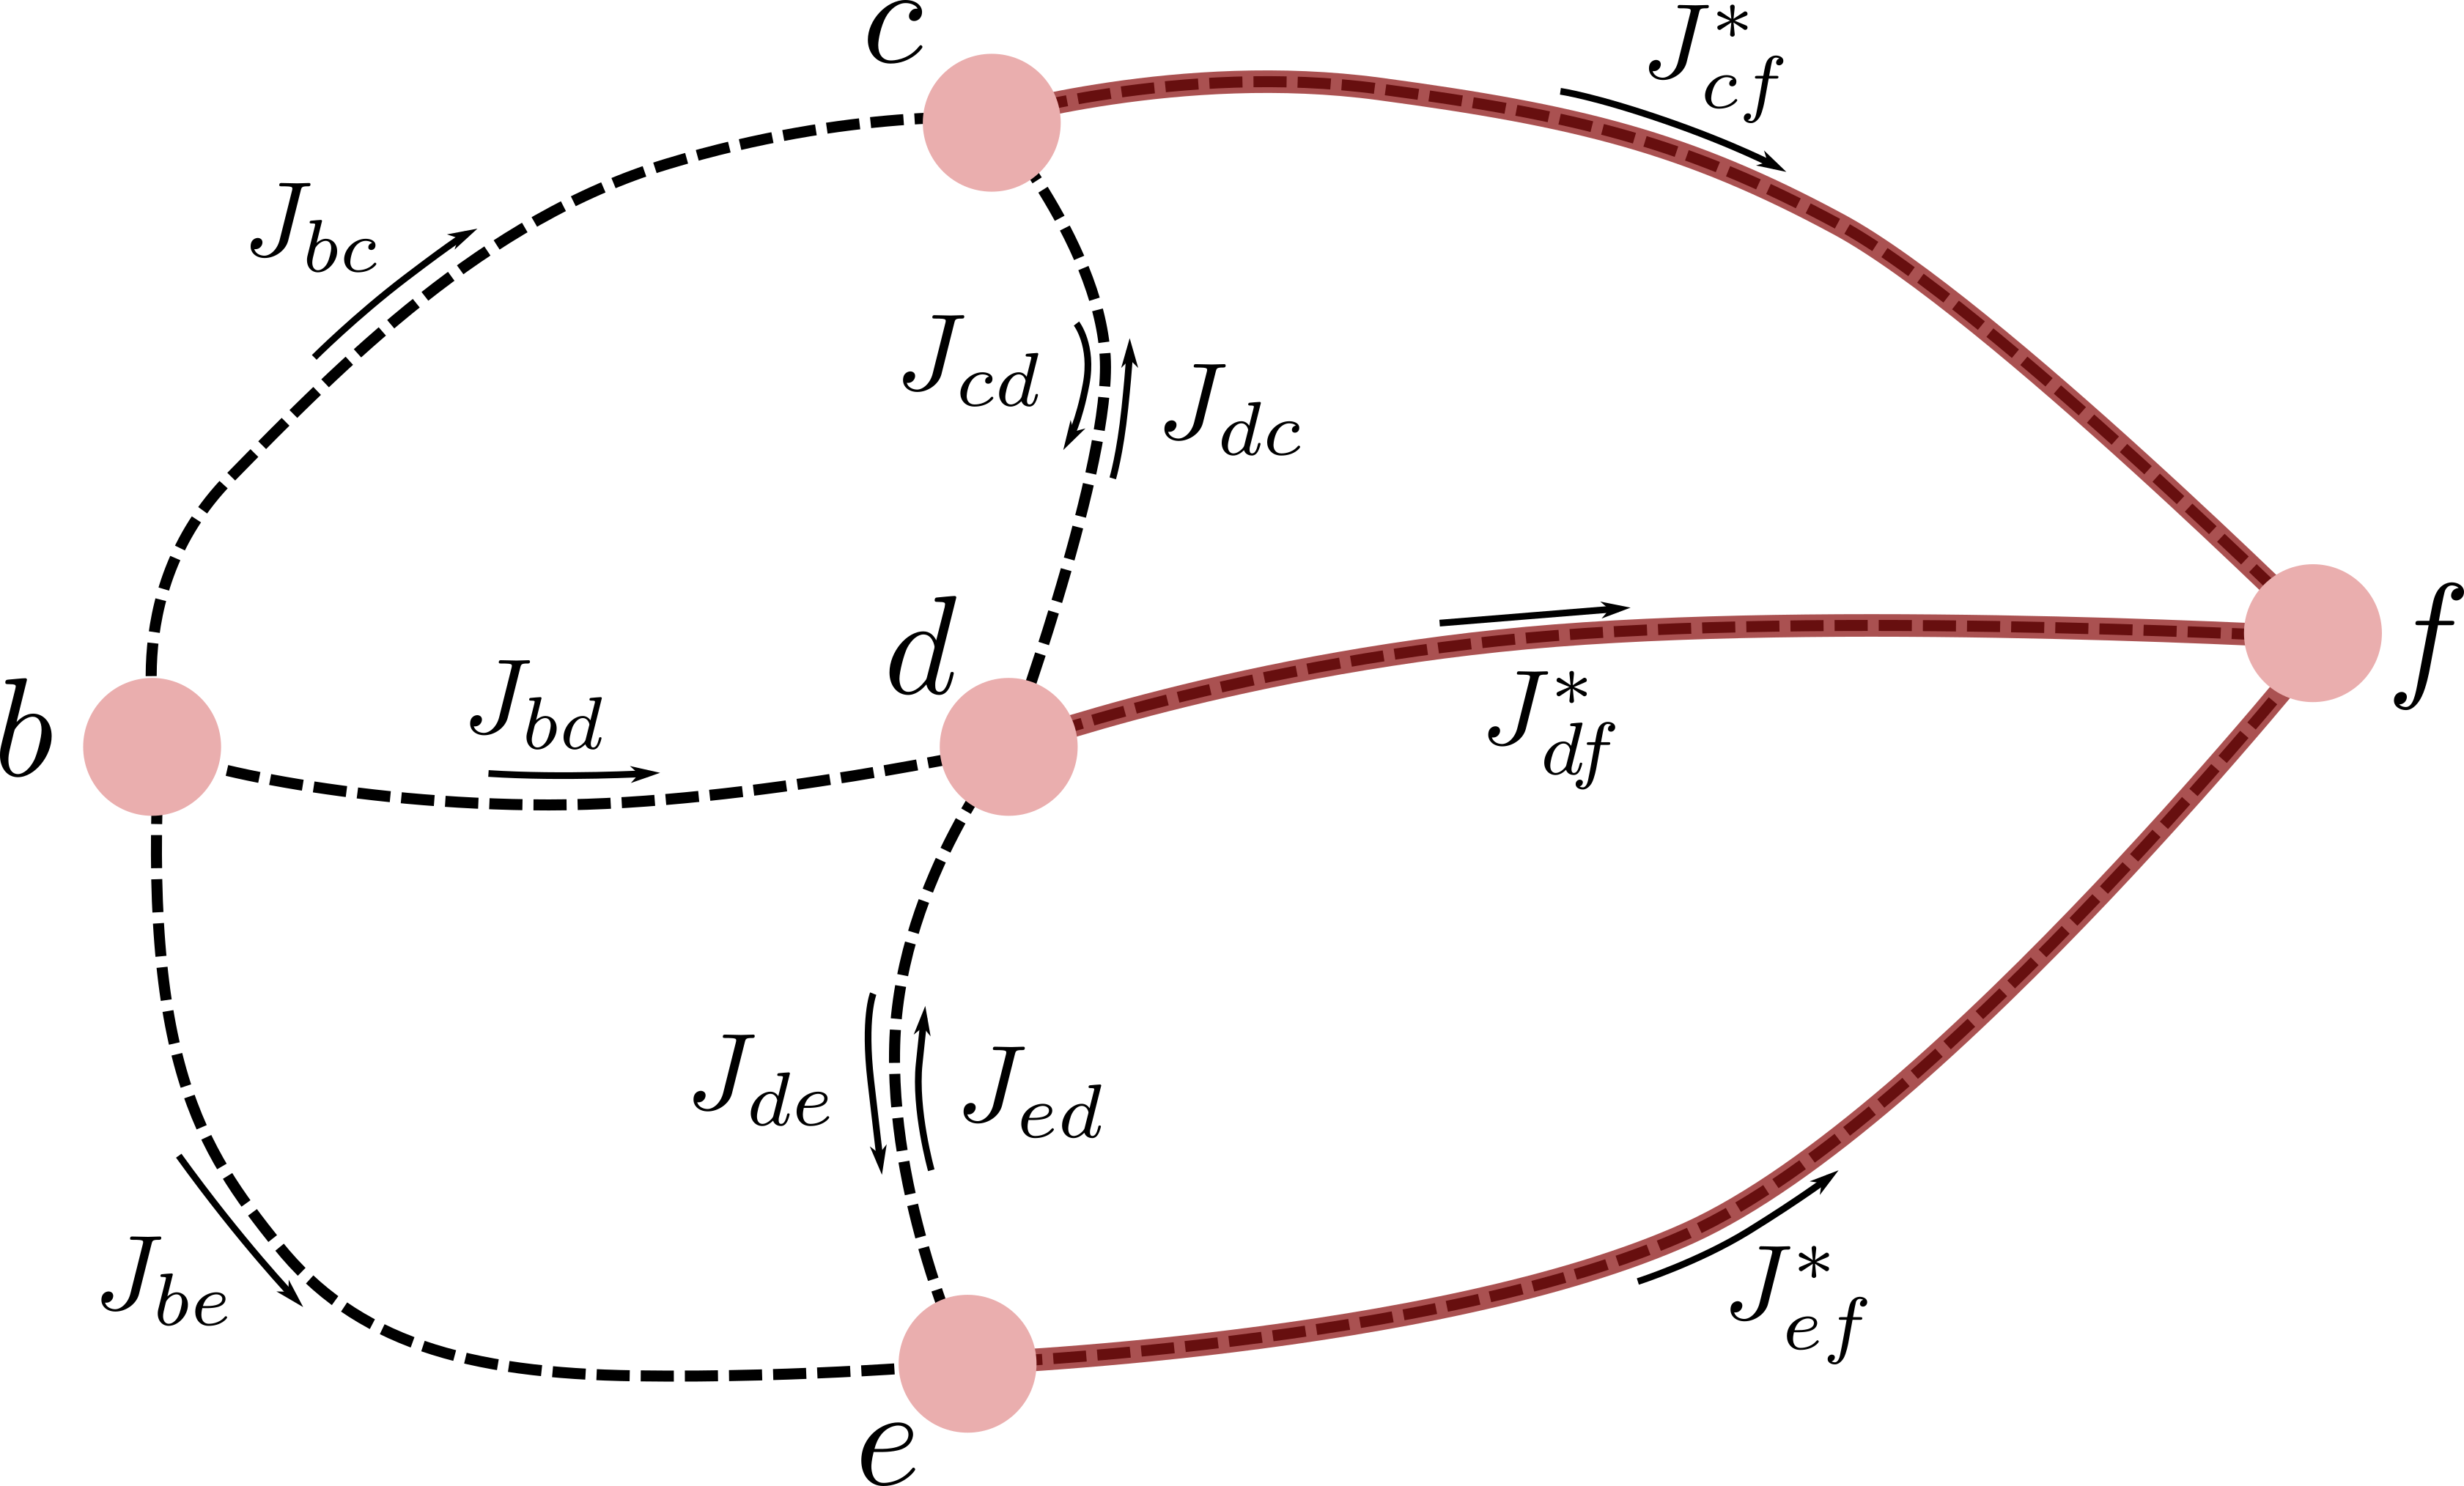
\includegraphics[width=0.65\textwidth]{tex/figs/ch22_figs/princopt2.png}
    \caption{Suppose the optimal paths from points $c$, $d$ and $e$ to $f$ are known (shown in green). By using the principle of optimality, an optimal path from point $b$ to $f$ can be found by \textit{only} searching over paths from $b$ to $c$, $d$, and $f$, and determining the lowest cost from the candidates $\{J_{bc} + J^*_{cf}, J_{bd} + J^*_{df}, J_{be} + J^*_{ef}\}$. In other words, the \textit{optimal tails} can be leveraged to reduce the total number of paths that need to be considered when finding an optimal path from $b$ to $f$!}
    \label{fig:princopt2}
\end{figure}

\subsubsection{Dynamic Programming (Deterministic)}
The dynamic programming (DP) algorithm \textit{globally} solves the deterministic decision making problem \eqref{eq:dproblem} by leveraging the principle of optimality\footnote[][4\baselineskip]{Note that the principle of optimality is a fundamental property that is actually utilized in almost all decision making algorithms, including reinforcement learning.}. The dynamic programming algorithm is given in Algorithm \ref{alg:dDP}, where it can be seen that a backward-in-time recursion is used and at each step a \textit{local} optimization is performed (this local optimization is referred to as the \textit{Bellman} equation), leveraging the optimal \textit{tail} costs from the previous iteration.
\begin{algorithm}[ht]
 $J^*_N(\x_N) = g_n(\x_N),$ for all $\x_N$\\
 \For{$k=N-1$ \KwTo $0$}{
  $J^*_k(\x_k) = \underset{\bu_k \in \mathcal{U}(\x_k)}{\min}g_k(\x_k,\bu_k) + J^*_{k+1}(f_k(\x_k, \bu_k)),$ for all $\x_k$\\
 }
 \Return $J^*_0(\cdot),\dots,J^*_N(\cdot)$
 \caption{Dynamic Programming (Deterministic)}
 \label{alg:dDP}
\end{algorithm}
The output of the dynamic programming algorithm is a set of costs $J^*_k(\x_k)$ for each time step $k = 0, \dots,N$ and states $\x_k$, which provide the optimal \textit{tail} cost for the \textit{tail} subproblem. 

Given an initial condition $\x_0$, the optimal control sequence $\{\bu^*_0,\dots,\bu^*_{N-1}\}$ that solves the deterministic decision making problem can be computed with a ``forward pass'', where:
\begin{equation*}
\bu_0^* = \underset{\bu_0 \in \mathcal{U}(\x_0)}{\arg \min}\:\:g_0(\x_0,\bu_0) + J^*_{1}(f_0(\x_0, \bu_0)).
\end{equation*}
The next state is then computed as $\x^*_1 = f_0(\x_0, \bu^*_0)$, and the process is repeated:
\begin{equation*}
\bu_1^* = \underset{\bu_1 \in \mathcal{U}(\x^*_1)}{\arg \min}\:\:g_1(\x^*_1,\bu_1) + J^*_{2}(f_1(\x^*_1, \bu_1)),
\end{equation*}
until the full trajectory and optimal control is specified.

Note that in practice the DP algorithm is not practical for continuously values states $\x$, since an infinite number of states would have to be iterated over. Therefore one possible modification to handle continuously valued states is to \textit{quantize} the state space into a finite set of states (other approaches, such as interpolation, are also possible). Also, it is interesting to note that the addition of control constraints can actually simplify the procedure, since it restricts the number of possible options that need to be considered!

\begin{example}[Deterministic Dynamic Programming] \label{ex:detDP}
\theoremstyle{definition}
Consider the environment shown in Figure \ref{fig:detDPprob}, where the goal is to start at point $a$ and reach point $h$ while incurring the smallest cost. In this problem the state is represented as the current location (i.e. $a$, $b$, etc.), and the control constraints are encoded by the arrows indicating possible directions of travel (e.g. at point $c$ it is possible to either go right or up, but not down or left). The cost of traversing between two points is also denoted in Figure \ref{fig:detDPprob}.
\begin{figure}[ht]
    \centering
    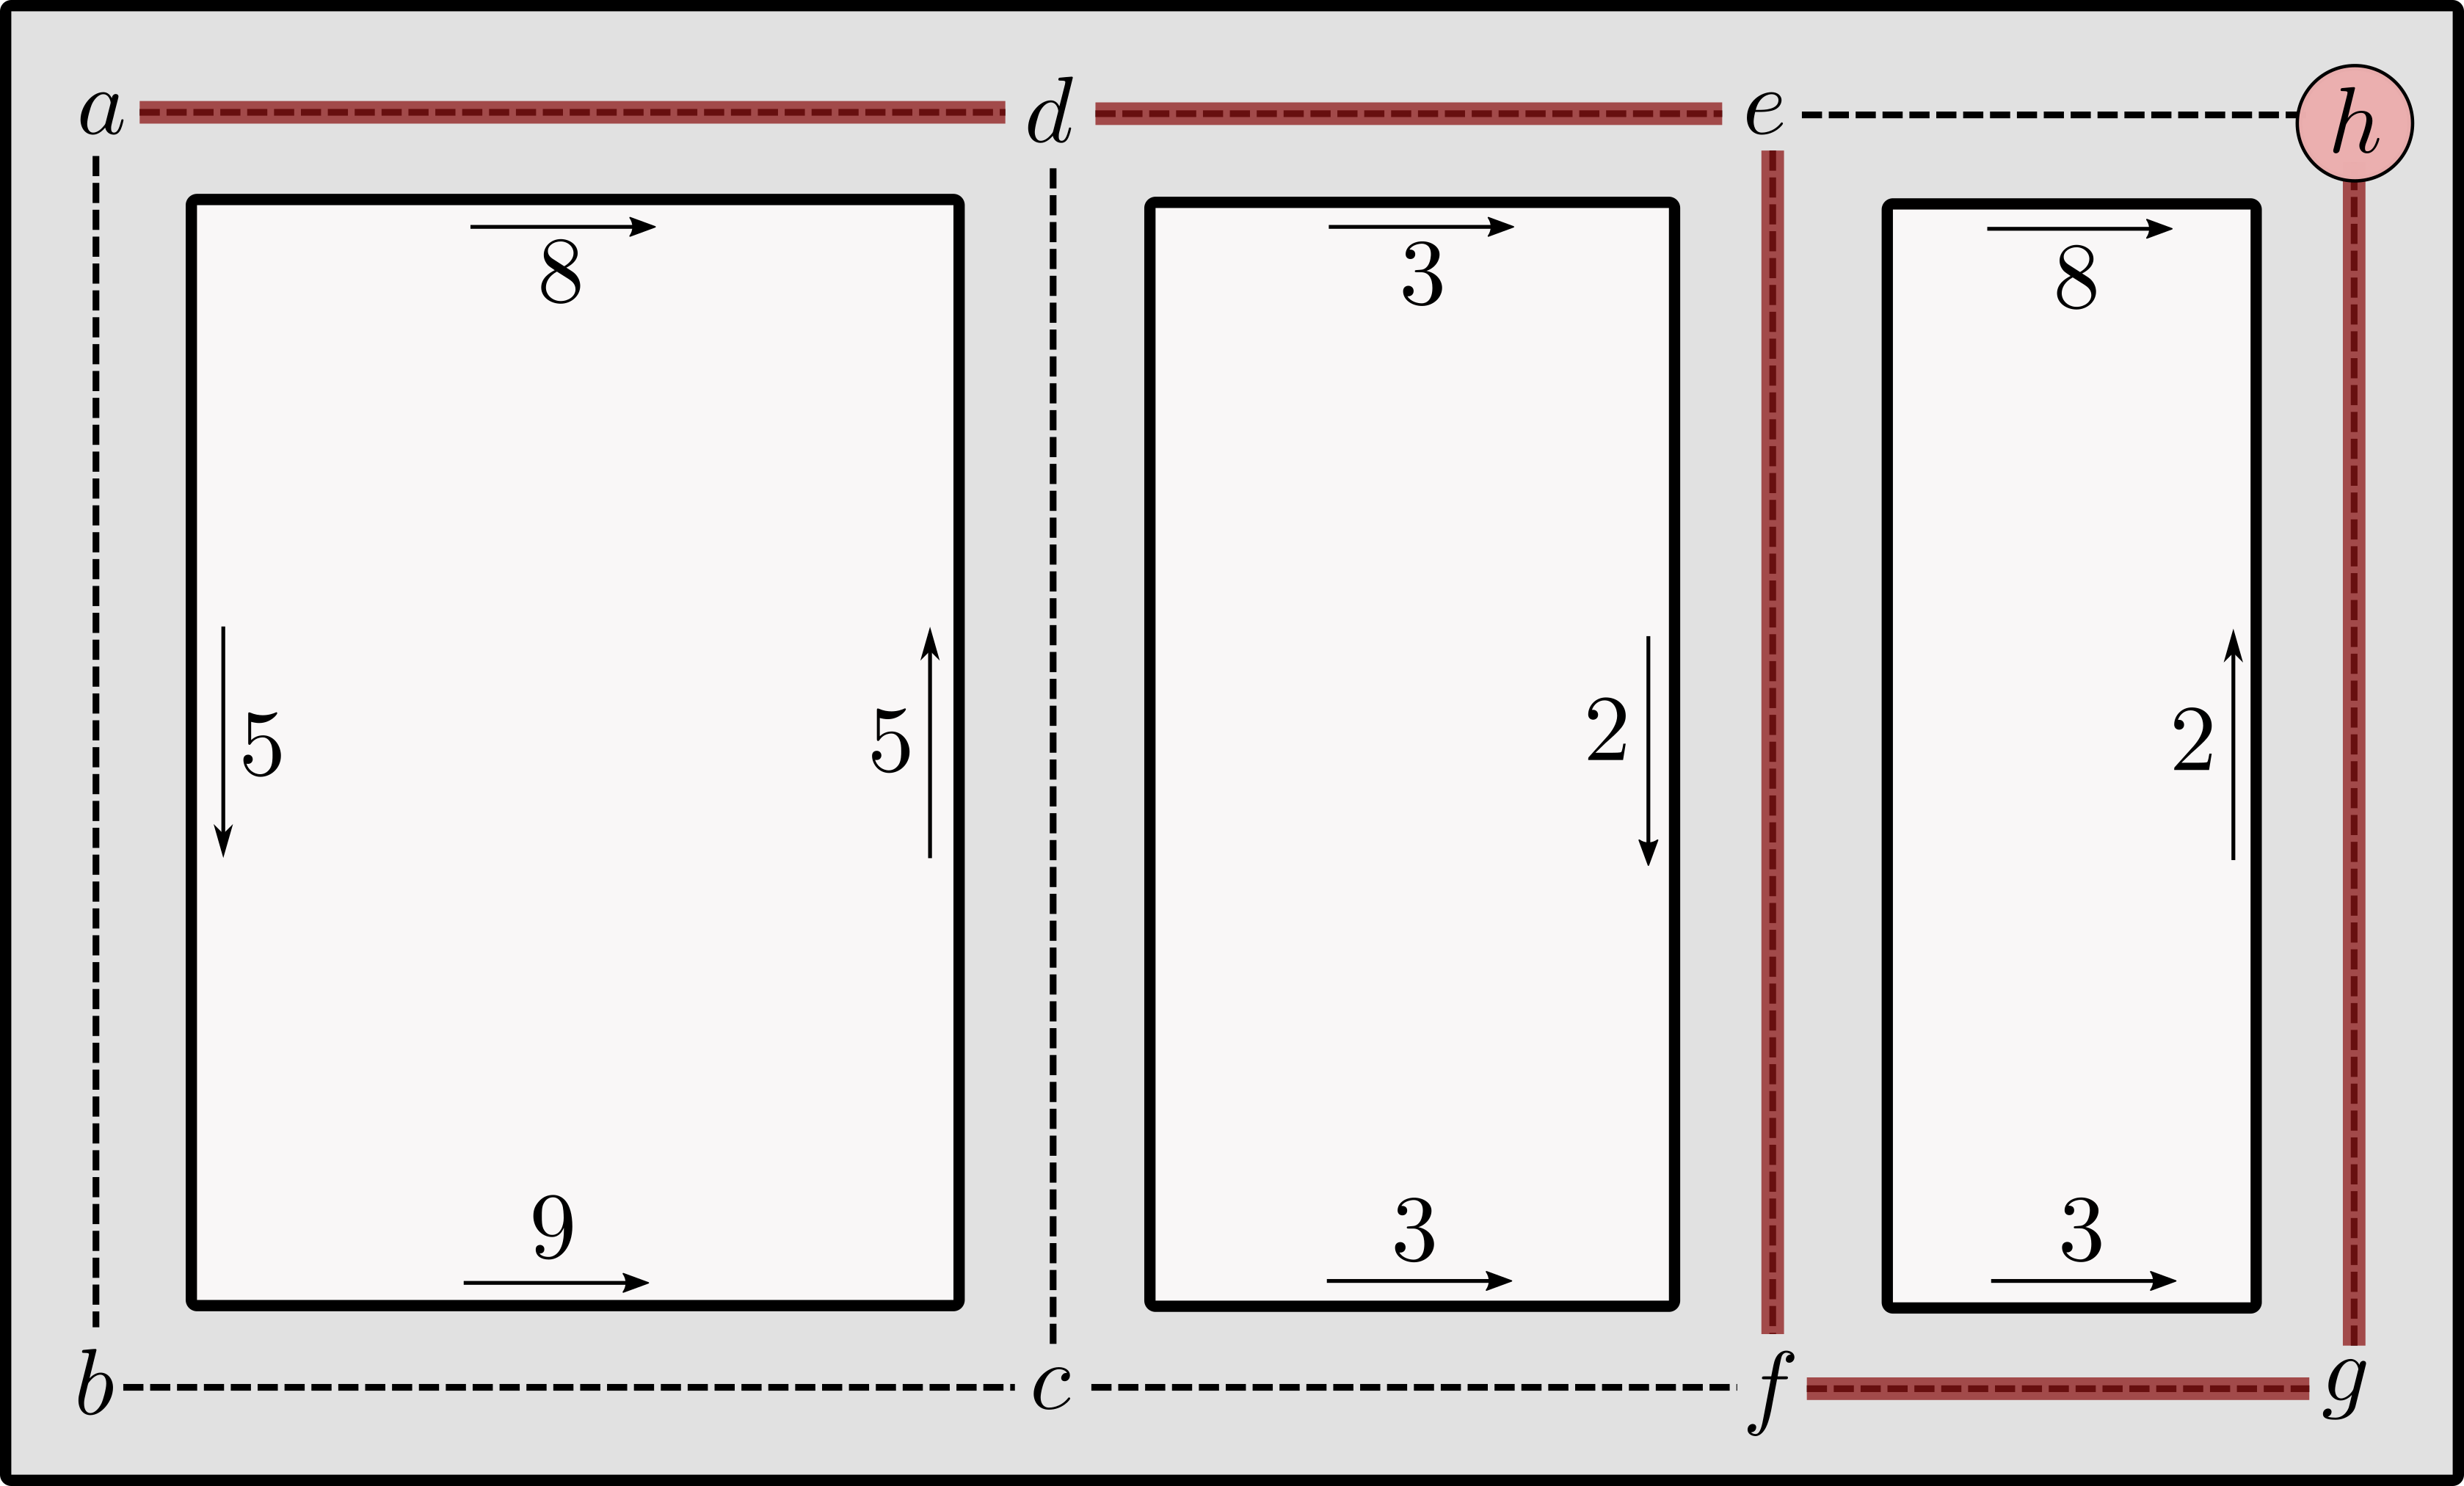
\includegraphics[width=0.8\textwidth]{tex/figs/ch22_figs/dpexample.png}
    \caption{A deterministic decision making problem where the goal is to move from point $a$ to point $h$ while incurring the minimal amount of cost. The green path indicates the optimal path. This problem is solved by dynamic programming in Example \ref{ex:detDP}.}
    \label{fig:detDPprob}
\end{figure}

To implement the DP algorithm, the final point $h$ is chosen as $\x_N$, and the DP recursion begins with:
\begin{equation*}
    J^*_N(h) = 0,
\end{equation*}
since there is no cost to stay at point $h$.
Moving backward in time, it can be seen that the possible states $\x_{N-1}$ that can transition to $\x_N = h$ are the points $h$, $e$, and $g$ (assuming it is possible to stay at $h$ with no cost). Therefore in the first step of the DP recursion:
\begin{equation*}
\begin{split}
J^*_{N-1}(h) &= 0 + J^*_N(h) = 0, \quad u^*_{N-1}(h) = \text{stay}. \\
J^*_{N-1}(e) &= 8 + J^*_N(h) = 8, \quad u^*_{N-1}(e) = \text{right}, \\
J^*_{N-1}(g) &= 2 + J^*_N(h) = 2, \quad u^*_{N-1}(g) = \text{up}, \\
\end{split}
\end{equation*}
Note that $J^*_k(h) = 0$ for all $k \leq N$, and therefore it will not be explicitly included in the following steps. In the next step:
\begin{equation*}
\begin{split}
J^*_{N-2}(e) &= 8 + J^*_{N-1}(h) = 8, \quad u^*_{N-2}(e) = \text{right}, \\
J^*_{N-2}(g) &= 2, \quad u^*_{N-2}(g) = \text{up}, \\
J^*_{N-2}(d) &= 3 + J^*_{N-1}(e) = 11, \quad u^*_{N-2}(d) = \text{right}, \\
J^*_{N-2}(f) &= 3 + J^*_{N-1}(g) = 5, \quad u^*_{N-2}(f) = \text{right}, \\
\end{split}
\end{equation*}
At this point, these optimal tail costs can be considered to be the optimal costs associated with control actions that lead from $e$, $g$, $d$, or $f$ to the end point $h$ in \textit{two} steps! Continuing on:
\begin{equation*}
\begin{split}
J^*_{N-3}(e) &= \min \{8 + J^*_{N-2}(h), \:2 + J^*_{N-2}(f)\} = 7, \quad u^*_{N-3}(e) = \text{down}, \\
J^*_{N-3}(g) &= 2, \quad u^*_{N-3}(g) = \text{up},  \\
J^*_{N-3}(d) &= 3 + J^*_{N-2}(e) = 11, \quad u^*_{N-3}(d) = \text{right}, \\
J^*_{N-3}(f) & = 5, \quad u^*_{N-3}(f) = \text{right}, \\
J^*_{N-3}(a) &= 8 + J^*_{N-2}(d) = 19, \quad u^*_{N-3}(a) = \text{right}, \\
J^*_{N-3}(c) &= \min \{5 + J^*_{N-2}(d), \:3 + J^*_{N-2}(f)\} = 8, \quad u^*_{N-3}(c) = \text{right}. \\
\end{split}
\end{equation*}
Interestingly, it can be seen that it is now possible to accomplish the objective (i.e. go from point $a$ to $h$) in 3 time steps (i.e. on path $a-d-e-f$) and incur an optimal cost of 19. However it turns out that an even lower cost is achievable if the number of time steps is increased further! Continuing the DP recursion:
\begin{equation*}
\begin{split}
J^*_{N-4}(e) & = 7, \quad u^*_{N-4}(e) = \text{down}, \\
J^*_{N-4}(g) &= 2, \quad u^*_{N-4}(g) = \text{up}, \\
J^*_{N-4}(d) &= 3 + J^*_{N-3}(e) = 10, \quad u^*_{N-4}(d) = \text{right}, \\
J^*_{N-4}(f) &= 5,  \quad u^*_{N-4}(f) = \text{right},\\
J^*_{N-4}(a) &= 8 + J^*_{N-3}(d) = 19, \quad u^*_{N-4}(a) = \text{right} \\
J^*_{N-4}(c) &= \min \{5 + J^*_{N-3}(d), \:3 + J^*_{N-3}(f)\} = 8, \quad u^*_{N-4}(c) = \text{right}, \\
J^*_{N-4}(b) &= 9 + J^*_{N-3}(c) = 17, \quad u^*_{N-4}(b) = \text{right},\\
\end{split}
\end{equation*}
and finally with one more iteration:
\begin{equation*}
\begin{split}
J^*_{N-5}(e) & = 7, \quad u^*_{N-5}(e) = \text{down}, \\
J^*_{N-5}(g) &= 2, \quad u^*_{N-5}(g) = \text{up}, \\
J^*_{N-5}(d) &= 10, \quad u^*_{N-5}(d) = \text{right}, \\
J^*_{N-5}(f) &= 5, \quad u^*_{N-5}(f) = \text{right}, \\
J^*_{N-5}(a) &= \min \{8 + J^*_{N-4}(d), \:5 + J^*_{N-4}(b)\} = 18, \quad u^*_{N-5}(a) = \text{right} \\
J^*_{N-5}(c) &= \min \{5 + J^*_{N-4}(d), \:3 + J^*_{N-4}(f)\} = 8, \quad u^*_{N-5}(c) = \text{right}, \\
J^*_{N-5}(b) &= 9 + J^*_{N-4}(c) = 17, \quad u^*_{N-5}(b) = \text{right}. \\
\end{split}
\end{equation*}
Additional iterations are not included in this example because the costs and optimal decisions will no longer change with longer horizons (see for yourself!). Therefore it can be seen that with a sufficiently long horizon ($N \geq 5$), the optimal path from $a$ to $h$ is $a-d-e-f-g-h$ and incurs a cost of $18$. Not this process has actually given a lot more information than what was original asked for. In particular, given \textit{any} starting point and \textit{any} horizon it is straightforward to generate an optimal control sequence! For example, if you wanted to start at point $c$ and get to $h$ in $N=3$ steps you could immediately see that the optimal path is $c-f-g-h$ and the optimal cost is $8$.
\end{example}


\subsection{Stochastic Decision Making Problem}
In the stochastic decision making problem it is assumed that there is some \textit{uncertainty} in the robot's behavior or in the environment. This uncertainty is captured in the stochastic discrete-time robot model:
\begin{equation} \label{eq:smodel}
\x_{k+1}= f_k(\x_k, \bu_k, \w_k), \quad k = 0, \dots, N-1,
\end{equation}
where $\w_k$ represents a stochastic disturbance term. Additionally, it is assumed that this disturbance has a known conditional probability distribution $P_k(\w_k \mid \x_k, \bu_k)$. Note that it is assumed that the disturbance is only dependent on the current state $\x_k$ and control $\bu_k$, and not states from earlier in the robot's history. This is another example of the Markov assumption, which was similarly used to develop the algorithms for localization and filtering in previous chapters.

Another main difference between the stochastic decision making problem and the deterministic problem is that a control \textit{policy} is computed in the stochastic case. A control policy, usually denoted $\bu = \pi(\x)$, is a function that maps the state $\x$ to a control $\bu$, and therefore defines a closed-loop controller (whereas in the deterministic setting an open-loop sequence was computed). Generally speaking, the search for control \textit{policies} makes the problem more difficult to solve, but is typically required in stochastic settings because uncertainty would lead to undesirable behavior under open-loop control plans. Specifically, in the stochastic decision making problem the policies $\pi = \{\pi_0, \dots, \pi_{N-1}\}$ are computed, which define the controls by $\bu_k = \pi_k(\x_k)$.

Of course the cost function is also modified to handle the uncertainty. In particular, a \textit{risk-neutral} formulation is used (i.e. minimize the cost \textit{on average}), where the cost is defined by the \textit{expected} value:
\begin{equation} \label{eq:scost}
J_\pi(\x_0) = E_{\w} \big[g_N(\x_N) + \sum_{k=0}^{N-1} g_k(\x_k, \pi(\x_k), \w_k)\big],
\end{equation}
where the expectation is over the stochastic variables $\w$. The stochastic decision making problem can now be stated as:
\begin{definition}[Stochastic Decision Making Problem]
The stochastic decision making problem can be expressed for the system model \eqref{eq:smodel}, control constraints \eqref{eq:SDMPconstraints}, and cost function \eqref{eq:scost} as:
\begin{equation} \label{eq:sproblem}
J^*(\x_0) = \underset{\pi}{\min} \:\:J_{\pi}(\x_0).
\end{equation}
\end{definition}


\subsubsection{Principle of Optimality (Stochastic)}
The principle of optimality can again be applied in the stochastic setting, and the intuition is identical to the deterministic case (however the proof is slightly different because the reasoning is in terms of probability distributions). The principle of optimality in the stochastic setting is stated formally as:
\begin{theorem}[Principle of Optimality (Stochastic)]
Let $\pi^* = \{\pi_0^*, \pi_1^* \dots, \pi_{N-1}^*\}$ be an optimal policy for the stochastic decision making problem \eqref{eq:sproblem}, and assume the state $\x_k$ is reachable. Then, the tail policy sequence $\{\pi_k^*, \dots, \pi_{N-1}^*\}$ is an optimal policy sequence when starting from $\x_k$ to minimize the cost from time $k$ to time $N$.
\end{theorem}
Again, by leveraging the principle of optimality the decision making problem can be simplified to making immediate decisions by concatenating optimal tail policies.

\subsubsection{Dynamic Programming (Stochastic)}
The dynamic programming algorithm for the stochastic setting is also quite similar to DP for deterministic problems, and is given in Algorithm \ref{alg:sDP}.
\begin{algorithm}[ht]
 $J_N(\x_N) = g_n(\x_N),$ for all $\x_N$\\
 \For{$k=N-1$ \KwTo $0$}{
  $J_k(\x_k) = \underset{\bu_k \in \mathcal{U}(\x_k)}{\min}E_{\w_k}\big[g_k(\x_k,\bu_k,\w_k) + J_{k+1}(f_k(\x_k, \bu_k, \w_k))\big],$ for all $\x_k$\\
 }
 \Return $J_0(\cdot),\dots,J_N(\cdot)$
 \caption{Dynamic Programming (Stochastic)}
 \label{alg:sDP}
\end{algorithm}
Once Algorithm \ref{alg:sDP} is run, the optimal policy is defined by:
\begin{equation*}
\pi^*_k(\x_k) = \underset{\bu_k \in \mathcal{U}(\x_k)}{\min}E_{\w_k}\big[g_k(\x_k,\bu_k,\w_k) + J_{k+1}(f_k(\x_k, \bu_k, \w_k))\big].
\end{equation*}

\begin{example}[Stochastic Dynamic Programming] \label{ex:stoDP}
\theoremstyle{definition}
Consider an inventory control problem, where the available stock of a particular item is the state $x_k \in \mathbb{N}$, the ability to add to the inventory is the control $u_k \in \mathbb{N}$, and the demand for the item is a stochastic variable $w_k \in \mathbb{N}$. The dynamics of the available stock is modeled as:
\begin{equation*}
x_{k+1} = \max \{0, x_k + u_k - w_k\},
\end{equation*}
which models the fact that demand reduces available stock but can also never be negative. Additionally, consider the control constraints:
\begin{equation*}
x_k + u_k \leq 2,
\end{equation*}
which limits the amount of additional inventory that can be added based on the current available stock to ensure that $x_k \leq 2$.
The demand $w_k$ is assumed to be modeled probabilistically with a distribution:
\begin{equation*}
p(w_k=0) = 0.1, \quad p(w_k = 1) = 0.7, \quad p(w_k = 2) = 0.2.
\end{equation*}
Finally, the cost is given for a horizon of $N=3$ as:
\begin{equation*}
E\big[\sum_{k=0}^2 u_k + (x_k + u_k - w_k)^2 \big],
\end{equation*}
which penalizes ordering new stock at each time step and also having available stock at the next time step (i.e. having to store stock).

The dynamic programming algorithm can then be applied, starting with the end costs:
\begin{equation*}
J_3(x_3) = 0,
\end{equation*}
and then recursively computing:
\begin{equation*}
\begin{split}
J_2(0) &= \underset{u_2 \in \{0,1,2\}}{\min} E\big[u_2 + (u_2 - w_2)^2  \big] = \underset{u_2 \in \{0,1,2\}}{\min} u_2 + 0.1u_2^2 + 0.7(u_2-1)^2 + 0.2(u_2 - 2)^2 = 1.3, \\
J_2(1) &= \underset{u_2 \in \{0,1\}}{\min} E\big[u_2 + (1 + u_2 - w_2)^2  \big] = 0.3,\\
J_2(2) &= E\big[(2 - w_2)^2  \big] = 1.1, \\
\end{split}
\end{equation*}
where the last cost is easily evaluated since the constraint makes $u_2 = 0$ the only feasible choice.
The optimal stage policies associated with this step are:
\begin{equation*}
\begin{split}
\pi^*_2(0) &= 1, \\ 
\pi^*_2(1) &= 0, \\ 
\pi^*_2(2) &= 0. \\ 
\end{split}
\end{equation*}
In the next step:
\begin{equation*}
\begin{split}
J_1(0) &= \underset{u_1 \in \{0,1,2\}}{\min} E\big[u_1 + (u_1 - w_1)^2 + J_2(\max\{0, u_1 - w_1\}) \big] = 2.5, \\
J_1(1) &= \underset{u_1 \in \{0,1,\}}{\min} E\big[u_1 + (1 + u_1 - w_1)^2 + J_2(\max\{0, 1 + u_1 - w_1\})  \big] = 1.5,\\
J_1(2) &= E\big[(2 - w_1)^2  + J_2(\max\{0, 2 - w_1\}) \big] = 1.68,\\
\end{split}
\end{equation*}
with optimal stage policies:
\begin{equation*}
\begin{split}
\pi^*_1(0) &= 1, \\ 
\pi^*_1(1) &= 0, \\ 
\pi^*_1(2) &= 0. \\ 
\end{split}
\end{equation*}
Finally, in the last step:
\begin{equation*}
\begin{split}
J_0(0) &= \underset{u_0 \in \{0,1,2\}}{\min} E\big[u_0 + (u_0 - w_0)^2 + J_1(\max\{0, u_0 - w_0\}) \big] = 3.7, \\
J_0(1) &= \underset{u_0 \in \{0,1,\}}{\min} E\big[u_0 + (1 + u_0 - w_0)^2 + J_1(\max\{0, 1 + u_0 - w_0\})  \big] = 2.7,\\
J_0(2) &= E\big[(2 - w_0)^2  + J_1(\max\{0, 2 - w_0\}) \big] = 2.818,\\
\end{split}
\end{equation*}
with optimal stage policies:
\begin{equation*}
\begin{split}
\pi^*_0(0) &= 1, \\ 
\pi^*_0(1) &= 0, \\ 
\pi^*_0(2) &= 0. \\ 
\end{split}
\end{equation*}
Interestingly, the best scenario occurs with an initial stock of one, rather than have no stock or too much stock. Also, the policy ends up being the same at all time steps: if you have no stock you add one item, otherwise you do nothing.
\end{example}

\subsection{Challenges and Extensions of Dynamic Programming}
Dynamic programming is a powerful algorithm, but suffers from several practical considerations: the ``curse of dimensionality'', the ``curse of modeling'', and the ``curse of time''. The curse of dimensionality arises because of a exponential growth of the computational and storage requirements based on the dimension of the state. For example if the state has dimension one (i.e. $\x \in \R$) and can take on 100 different values, then at each step of the algorithm the Bellman equation must be solved 100 times. While this may be possible from a practical perspective, if $\x \in \R^3$ this would lead to $100^3$ solves of the Bellman equation! Additionally, extensions to the problems presented in this chapter where the full state is not \textit{known} (e.g. because you can only measure some parts of the state), the problem also become intractable. The curse of modeling results from the complexity of modeling stochastic systems. In particular, it can be very hard to obtain expressions for transition probabilities for real world systems! Lastly, the curse of time is that the data of the problem may not be known ahead of time (such that the DP algorithm can be run offline). Therefore it may be required to solve the DP algorithm online when the data becomes available, or when the data changes and the problem needs to be resolved.

\subsubsection{Reinforcement Learning}
The practical challenges related to dynamic programming motivated the development of \textit{suboptimal} dynamic programming approaches, which more commonly are referred to as \textit{reinforcement learning} approaches. The goal of these approaches is to make \textit{approximations} to the original problem that make it more practical for specific settings, such as with high-dimensional states, when the model is not known, and more. Broadly speaking, there are two main categories of approximations. The first category includes approximations in the value space (i.e. where the optimal cost function is approximated). The second category includes approximations in the policy space (i.e. where the policy is approximated by a neural network whose weights are optimized over).


